\documentclass{article}[11pt,a4,twosided,doublespacing,titlepagenumber=on,numbers=endperiod]
\usepackage[utf8]{inputenc}
\usepackage[margin=2cm]{geometry}
%\usepackage{texcount}
%\usepackage[round,authoryear,sort]{natbib}
\usepackage[colorlinks=false,pdfborder={0 0 0},plainpages=false,pdfpagelabels]{hyperref}
\usepackage{setspace}
\usepackage{float}
\usepackage{graphicx}
\usepackage{svg}
\usepackage{amsmath} 
\usepackage{booktabs}


\title{Miniproject report: Model fitting of functional response curves}
\author{wz2812 }
\date{March 2020}

\begin{document}

\maketitle

\newpage

\renewcommand{\contentsname}{Table of Contents}
\tableofcontents
\newpage

\section{Introduction}
\doublespacing
A functional response in ecology introduce the relationship between the intake rate of a consumer and the density of the target resource. Numerical response and functional response are associated with each other, both used to describe the reproduction rate and population change as a function of the resource density. Functional responses can also be applied to determine the stability of food webs in various ecosystems. Functional responses are classified into three basic types first by C.S. Holling \cite{holling1959components}. Therefore, they are usually called Holling's type I, II, and III functional response.
\begin{figure}[H]
\centering
%\graphicspath{{../Data/}}
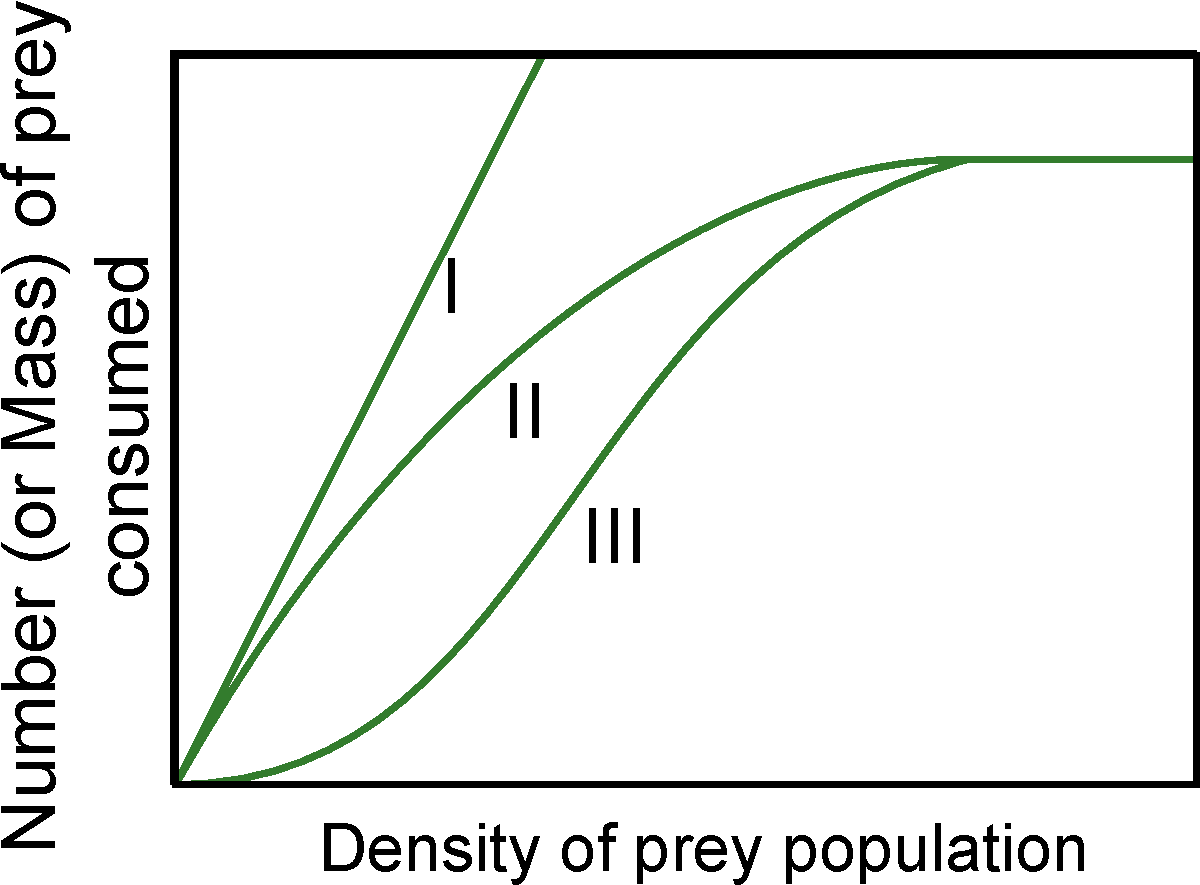
\includegraphics[height= 60mm]{../Data/FR.pdf}
\renewcommand\thefigure{\arabic{figure}}
\setcounter{figure}{0}
\caption{Holling's type I, II, and III functional responces}
\end{figure}
\noindent Type I functional response assumes proportional linear increase in consumption rate with resource density. And only when resource density increase to maximum, the consumption rate stops increasing and remains constant beyond that point. This implies a straight forward formula
\begin{equation}
    c = a x_R
\end{equation}
where $c$ is the consumption rate, $a$ is the search rate, and $x_R$ is the resource abundance.\\
\noindent
A type II functional response is a non-linear model proposed by Holling on the basis of separating a consumer's time into two activities:`searching resource' and `handling resource'\cite{dawes2013derivation}. As the consumption rate increase, more resource consumed requires more time to handle, which leads to a decrease in the total time for searching resource. Combining this with type I model leads to 
\begin{equation}
    c = \frac{a x_R}{1+ h a x_R}
\end{equation}
where $h$ is handling time of the consumer for that resource. By this formula, saturation occurs at high levels of resource density, and consumption rate remains constant after that saturation point.\\
\noindent
Type III functional response can be considered as a generalisation of the type II response to the form 
\begin{equation}
    c = \frac{a {x_R}^{q+1}}{1 + h a {x_R}^{q+1}}
\end{equation}
with $q$ to be a shape parameter for the response. The type III response is motivated by the learning behaviour of the consumers, while there is a learning time for them to improve of their success rate in searching and attacking. This leads to a slow increase in the consumption rate at low resource density levels, and an accelerating step as consumers meeting more resources until they fulfill their `skills'.\\
\noindent
Apart from Holling's type responses, there are also some more mechanistic approaches for the functional response such as Beddington-DeAngelis functional response\cite{cantrell2001dynamics}\cite{geritz2012mechanistic}.


\section{Methods}
\subsection{Dataset}
The dataset is called $CRat.csv$. It has 4507 observations each with 68 different measurements including rates of consumption of a single resource species by a consumer species. Consumption rate and resource density in functional response are also collected into this dataset as $N\_TraitValue$ and $ResDensity$ respectively. Each individual functional response curves can be identified by filtering the dataset by the same $ID$ values. Alternative ways are to reconstruct them by the same $Citation$ values or consumer/resource species ID.\\
\noindent
$N\_TraitValue$ is the consumption rate in each observation, which is in terms of biomass quantity or number of individual resource consumed per unit time per unit consumer.
\\
\noindent
$ResDensity$ is the resource density, which is in terms of biomass quantity or number of individual resource per unit area or per unit volume. \\
\noindent
$ID$ is the ID number of individual consumer, there are 308 unique individual consumer in the dataset. The unique number of different citations and consumer/resource species ID are 113, 125, and 123 respectively. In addition, observations of each unique individual consumer are collected from the same citation with same consumer and resource species ID. Consumption rate unit and resource density unit also vary between different ID values. Therefore, fitting individual functional response curves by ID values will fit more curves and tends to be more precise.

\subsection{Data preparation}
In data preparation step, I use a python file $data\_preparation.py$ to read the $CRat.csv$, and try to remove some obviously wrong observations which may affect model fitting results. In this case I just simply remove all observations with negative values and NAs from the columns we will use later, which is $N\_TraitValue$, $ResDensity$, and ID. Only filtering these three columns that will be used in model fitting, and finally write them into a new csv file called $data.csv$.

\subsection{Model introduction}
Many mathematical approaches can be applied into functional responses problems, non-linear least squares is one of the most well-known methods. Non-linear least squares is a form of non-linear regression using least squares analysis to fit $m$ observations with a non-linear model with $n$ unknown parameters ($m >= n$). It is widely used since it is fundamental and quick to fit\cite{cadet2006quantitative}. \\
\noindent
Two main fields of interest in functional responses problems are consumption rate the resource density. From the simplest non linear model to intermediate functional response model, a total of four different models will be fitted and computed. Further analysis is also used to test the performance of these models. \\
\noindent
The first two models are the simplest non-linear approach: quadratic and cubic polynomial models
\begin{equation}
    y = a x^2 + b x + c
\end{equation}
\begin{equation}
    y = a x^3 + b x^2 + c x + d
\end{equation}
where $y$ and $x$ in functional responses problems are consumption rate and resource density. These models are trivial, but simple to fit and also essential in model fitting. Many of the complicated statistical models ends up to be overfitted, simple models are widely used as a basic reference in model comparing.
The rest models are the two classical functional response models mentioned previously. The Holling type II model
\begin{equation}
    c = \frac{a x_R}{1+ h a x_R}
\end{equation}
and the generalised Holling model
\begin{equation}
    c = \frac{a {x_R}^{q+1}}{1 + h a {x_R}^{q+1}}
\end{equation}
This model is a generalised form of the Holling type functional responses, with an additional parameter $q$ which does not have any biological meaning. From the previous introduction of Holling's functional responses, when the handling time is not considered ($h = 0$):
\begin{equation}
    c = a x_R
\end{equation}
this is a Holling's type I functional response, and obviously when $q = 0$ it is a Holling's type II response as equation (6). Also when $q$ is positive, the consumption increase slowly at low resource density levels, introducing a learning behaviour for the consumers, which is exactly a Holling's type III response. \\
\noindent Each model above will fit a functional response curve for each individual identified by different ID values of the data. 

\subsection{Calculate starting value}
The main challenge in NLLS fitting is finding the right starting values. A unique starting value need to be determined for each individual functional response for each model. Algorithms are essential to generate large number of functional responses for parameters in each model.\\
\noindent
In quadratic and cubic models, the starting value can be simple since they are likely to fit in most cases. The parameters in these models are the coefficients of the polynomials $a$, $b$, $c$, and $d$. In model fitting step, I consider all the starting value of these parameters to be a random normal distribution, with mean to be the same as the mean in dataset and variance $1$.\\
\noindent
Holling's type II model has two parameters, the consumer's search rate $a$ and the resource handling time $h$. Similar approach has been made to search rate by Samraat et al.\cite{pawar2012dimensionality}, using machanistic model to define search rate of the functional response in terms of body size of consumers and resources
\begin{equation}
    a = s_D v_r d^{D-1}
\end{equation}
with $v_r$ and $d$ to be the searching speed and searching radius. In our dataset, there is no precise data of body size and searching radius, so I find the starting search rate $a$ from the data by calculating the steepest gradient of the consumption rate increase with resource density. The consumption rate saturates at high levels of resource density. From the equation (2) of the Holling type II model, when $x_R$ goes to $\infty$ the consumption rate will tends to be $1/h$. Therefore, the handling time $h$ can be determined by the asymptotic consumption rate. More precisely, the asymptotic consumption rate is simply considered as
\begin{equation}
    c_{asy} = c_{max} + \frac{1}{2} (c_{max} - c_{\text{second largest}})
\end{equation}
that implies
\begin{align*}
    h &= \frac{1}{c_{asy}}\\
      &= \frac{1}{c_{max} + \frac{1}{2} (c_{max} - c_{\text{second largest}})}
\end{align*}
Similar to Holling type II model, the generalised Holling model have the same parameters $a$ and $h$, but the additional parameter $q$ is also used from the equation (3) as the shape parameter determines the dimension of the resource density. The starting values of $q$ is set to be a random uniform distribution from 0 to 3. This value satisfies a clear separation from the Holling's type II model and also prevents fitting failure when the dimension of the resource density to be too large.

\subsection{Model fitting}
Once the starting values and data are all set, model fitting process will not be difficult. The main fitting step is accomplished in $R$ using function $nlsLM$ in package minpack.lm\cite{elzhov2016package}. This function is a modified version of non-linear fitting which is available for most of the generic function used in model analysis(e.g AIC, BIC). The model with the most parameter have 4 different parameters, which by definition of non-linear least squares requires at least 4 observation to fit. In my model fitting step, I only consider the ID values with 5 or more observations which will not cause bad fitted results due to lack of observations. \\
\noindent
For a total of 308 different individuals' data, the four models are fitted every time with unique calculated starting values of their parameters. Some mechanistic models are unlikely to fit for all individuals' data, so it is essential to use $tryCatch$ to prevent error popping up during model fitting. However, about 40\% of the individuals is going to fail fitting in at least one model by this method. To increase the fitting success rate, different starting values are worth trying. Given some of the starting values of parameters in the model are determined by a distribution which varies every time, we can keep the fitting process until it is fitted correctly. Using this technique, a upper bound number is required for each fitting loop. Also for parameters $a$ and $h$ with fixed starting values in each individual, random numbers close to the fixed values can be considered within each loop. I accept a random number within 20\% error of the fixed starting value for both $a$ and $h$ in the model fitting. Using the parameters of fitted models, we can predict the fitted observations of the dataset and record the predicted consumption rate in each observation for each model for future plotting. Statistical measures AIC, BIC and $R^2$ are calculated for model comparison and analysis.

\subsection{Computing tools}
There are two shell scripts used in the project: one to compile the pdf from the tex file, and a bash script runs the whole project and all other python and R files. \\
\noindent
Python is used in data preparation step and the only package used is $pandas$ for reading and writing csv dataset.\\
\noindent
R is the main computing tool in this project. NLLS fitting, plotting and analysis are all done in R within different files. In NLLS fitting, $minpack.lm$ is the main package used for model fitting. $ggplot2$ is the main package used in plotting, it is a great tool to visualise the data in R.

\newpage

\section{Plotting and results}
Using non-linear least squares fitting, 4507 observations of consumption rate are all fitted with four different models. Each individual with correctly fitted models can plot a prediction line for the fitted curve using $ggplot$.
\begin{figure}[H]
\centering
%\graphicspath{{../Data/}}
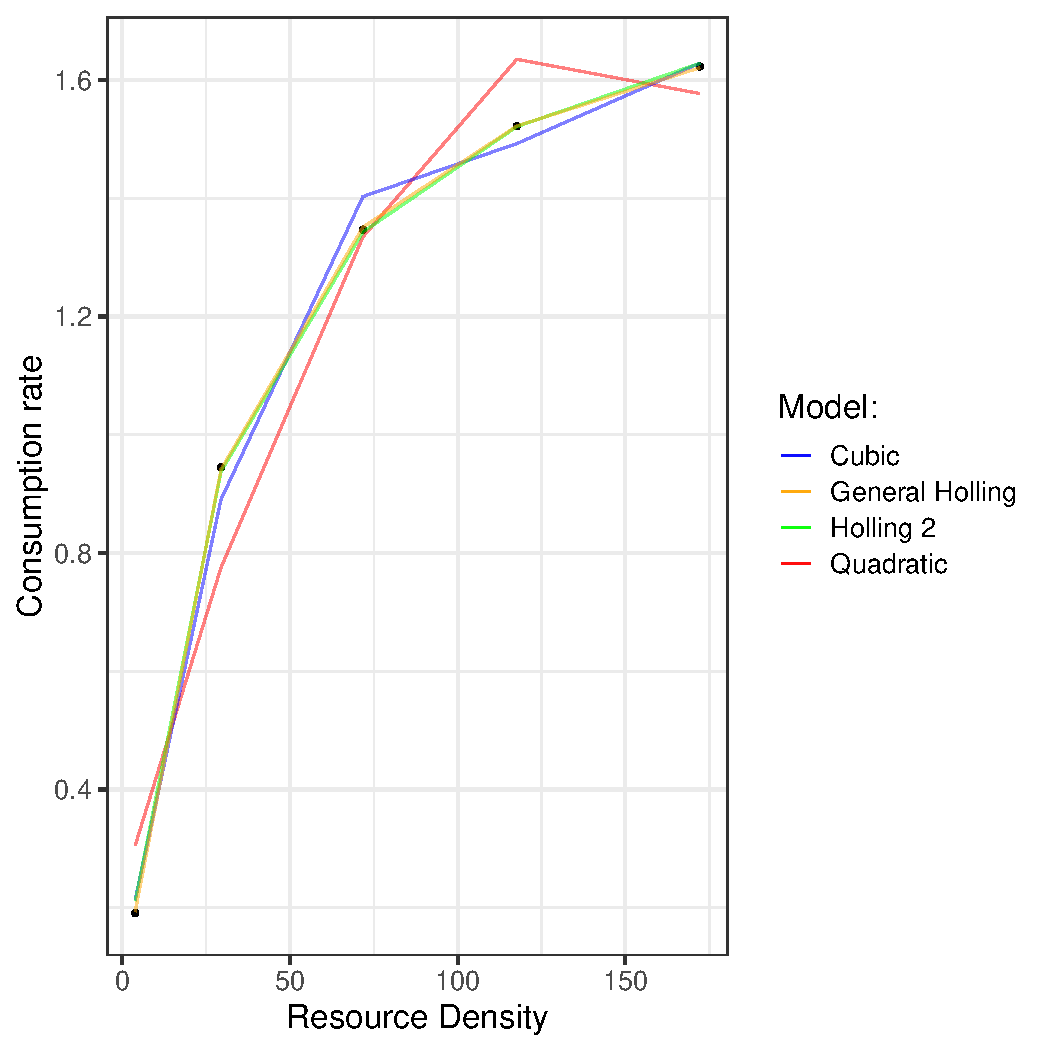
\includegraphics[height= 60mm]{../Results/plot/Functional_response_curve_40130.pdf}
\renewcommand\thefigure{\arabic{figure}}
\setcounter{figure}{0}
\caption{Need a finished plot with ID number}
\end{figure}
\noindent However, not all individuals can be fitted nicely by all the models. Lack of observations for each individual, outliers and bad observation results are the main reason causing failure in fitting. In the end among 308 individuals, 13 individuals are filtered out due to lack of observations. 

\begin{table}[H]
\centering 
\begin{tabular}{l c c c c}
\toprule % Top horizontal line
& \multicolumn{4}{c}{\textbf{Fitted models}} \\
\cmidrule(l){2-5}
\textbf{Individuals} & Quadratic & Cubic & Holling's Type II & Generalised Holling\\ % Column names row
\midrule % In-table horizontal line
Fitted & 295 & 294 & 234 & 231\\ % Content row 1
Total  & 295 & 295 & 295 & 295\\ % Content row 2
%PPD234 & 0.915 & 0.936 & 0.491 & 0.276 0.965\\ % Content row 3
%JSB126 & 0.828 & 0.827 & 0.528 & 0.518 0.926\\ % Content row 4
%JSB724 & 0.916 & 0.933 & 0.482 & 0.644 0.937\\ % Content row 5
\midrule % In-table horizontal line
\midrule % In-table horizontal line
Success Rate & 100\% & 99.6\% & 79.3\% & 78.3\% \\ % Summary/total row
\bottomrule % Bottom horizontal line
\end{tabular}
\caption{Number of individuals fitted and the success rate for each model in model fitting} % Table caption, can be commented out if no caption is required
\label{tab:template} % A label for referencing this table elsewhere, references are used in text as \ref{label}
\end{table}
\noindent
The fitting table for the rest of 295 individuals implies that quadratic and cubic polynomials are simple to fit with a extremely high percentage of success rate. On the other hand, models of functional responses share similar success rate, while generalised form of Holling's functional response are only slightly harder to fit than the more specific type II model.

\section{Analysis and discussion}
To examine the results in a statistical way, AIC, BIC and the coefficient of determination (R squared) for all individuals are recorded during the model fitting process. The Akaike information criterion (AIC) is an estimator of data, describing the quality of the in statistical modelling. The value of AIC is determined by number of parameters and the maximum value of the likelihood function with the formula
\begin{equation}
    \text{AIC} = 2k - 2 ln(\widehat{L}) 
\end{equation}
\noindent
Similarly, the Bayesian information criterion (BIC) is defined as
\begin{equation}
    \text{BIC} = ln(n)k - 2 ln(\widehat{L}) 
\end{equation}
where $k$ is the number of parameters, $\widehat{L}$ is the maximum likelihood, and $n$ is the number of observations in data. Both of them deal with the trade off between the goodness of fit and the simplicity of the model. The sample size for each individual is relatively small in my data. AIC value will not change with the number of observation in data, but it has a modification for small sample sizes AICc with
\begin{equation}
    \text{AICc} = \text{AIC} + \frac{2k^2 + 2k}{n - k -1}
\end{equation}
In this project I will use AIC to analyse the performance of models and compare that with AICc and discuss the results. The model with smaller AIC value is the better fit, so for each individual I find the best model with the minimum AIC value and models with AIC values difference less than 2 from the minimum AIC will all considered as they are equally the best. At last, count the total number of best fit for each model and compare results.

\begin{table}[H]
\centering 
\begin{tabular}{l c c c c}
\toprule % Top horizontal line
& \multicolumn{4}{c}{\textbf{Fitted models}} \\
\cmidrule(l){2-5}
\textbf{AIC} & Quadratic & Cubic & Holling's Type II & Generalised Holling\\ % Column names row
\midrule % In-table horizontal line
Best fit & 146 & 220 & 93 & 138\\ % Content row 1
Total fit  & 295 & 294 & 234 & 231\\ % Content row 2
Number of parameters & 3 & 4 & 2 & 3\\ % Content row 3
%JSB126 & 0.828 & 0.827 & 0.528 & 0.518 0.926\\ % Content row 4
%JSB724 & 0.916 & 0.933 & 0.482 & 0.644 0.937\\ % Content row 5
\midrule % In-table horizontal line
\midrule % In-table horizontal line
Best fit rate & 49.5\% & 74.8\% & 39.7\% & 59.7\% \\ % Summary/total row
\bottomrule % Bottom horizontal line
\end{tabular}
\caption{Best fit rate among models using AIC} % Table caption, can be commented out if no caption is required
\label{tab:template} % A label for referencing this table elsewhere, references are used in text as \ref{label}
\end{table}
\noindent
The table above illustrates two main problems in our case when applying AIC: the best fit rate are highly related to the number of parameters, which AIC is highly likely to overfit. Also some individuals can also fitted by quadratic and cubic model, which makes best fit in these individuals less competitive. Therefore, I improve the table using AICc instead, and only find the best fit among those individuals can be fitted by all of the models.

\begin{table}[H]
\centering 
\begin{tabular}{l c c c c}
\toprule % Top horizontal line
& \multicolumn{4}{c}{\textbf{Fitted models}} \\
\cmidrule(l){2-5}
\textbf{AICc} & Quadratic & Cubic & Holling's Type II & Generalised Holling\\ % Column names row
\midrule % In-table horizontal line
Best fit & 69 & 43 & 145 & 78\\ % Content row 1
Total fit  & 231 & 231 & 231 & 231\\ % Content row 2
Number of parameters & 3 & 4 & 2 & 3\\ % Content row 3
%JSB126 & 0.828 & 0.827 & 0.528 & 0.518 0.926\\ % Content row 4
%JSB724 & 0.916 & 0.933 & 0.482 & 0.644 0.937\\ % Content row 5
\midrule % In-table horizontal line
\midrule % In-table horizontal line
Best fit rate & 29.8\% & 18.6\% & 62.8\% & 33.8\% \\ % Summary/total row
\bottomrule % Bottom horizontal line
\end{tabular}
\caption{Best fit rate among models using AICc} % Table caption, can be commented out if no caption is required
\label{tab:template} % A label for referencing this table elsewhere, references are used in text as \ref{label}
\end{table}
\noindent
The best fit rate changes completely after using AICc instead of AIC. It turns out cubic model is just overfitting with small sample sizes and the Holling's type II is the best model among them with almost double the best fit rate of the generalised Holling model. \\
\noindent
R square value is the proportion of the variance in the dependent variable from independent variable. It varies from $-\infty$ to 1, and the closer it gets to 1, the better the fitting. However, R square values are not often used in determine the goodness of fitted models since they do not indicate whether a regression model is adequate. For 4 different models, the averaging R square values of cubic polynomial is the highest, following by quadratic, generalised Holling's response and Holling's type II response. This is also because the various number of parameters. Therefore R square is not a good reference for testing the goodness of fit in this case.





since the sample size for each individual is relatively small 
R square\\
discussion\\
(addressing biological questions involving co-variates)
\newpage

%\renewcommand\bibname{Bibliography}
%\addcontentsline{toc}{chapter}{\bibname}
%\bibliographystyle{abbrvnat}
%\bibliography{bibtexfile}
\phantomsection
\renewcommand\refname{Bibliography}
%\addcontentsline{toc}{section}{\bibname} % Add an entry for the Bibliography in the Table of Contents
%\pagestyle{headings}
\bibliographystyle{IEEEtran} % set the bibliography style
\bibliography{bibtexfile}

\end{document}
